\section{Specification}
The following chapter describes the implementation of the application.
\subsection{Main window}
The main window is divided into two parts, see figure \ref{fig:mainwindow}. On the very top of the application is a menubar where the user can do actions like saving their work. Then the window is split up in two parts. On the left side is the menubar and on the right side the grid. The grid is the representation of the traffic situation. The components (see section \ref{sec:components}) can be dragged from the sidebar to the grid. To remove a component right-click on it and press on Delete in the context-menu. All open incoming lanes have a text-box which allows the user to specify the amount of traffic coming. The simulation can simply be started by the play button and the simulation speed can simply be changed with a slider. With the button "Show Report" the user can get a report of that moment of the simulation. The report will contain a still image of the current situation. It highlights the traffic jams and the image can be saved.

\begin{figure}[!ht]
	\caption{Mockup of the Main window}
	\label{fig:mainwindow}
	\centering
	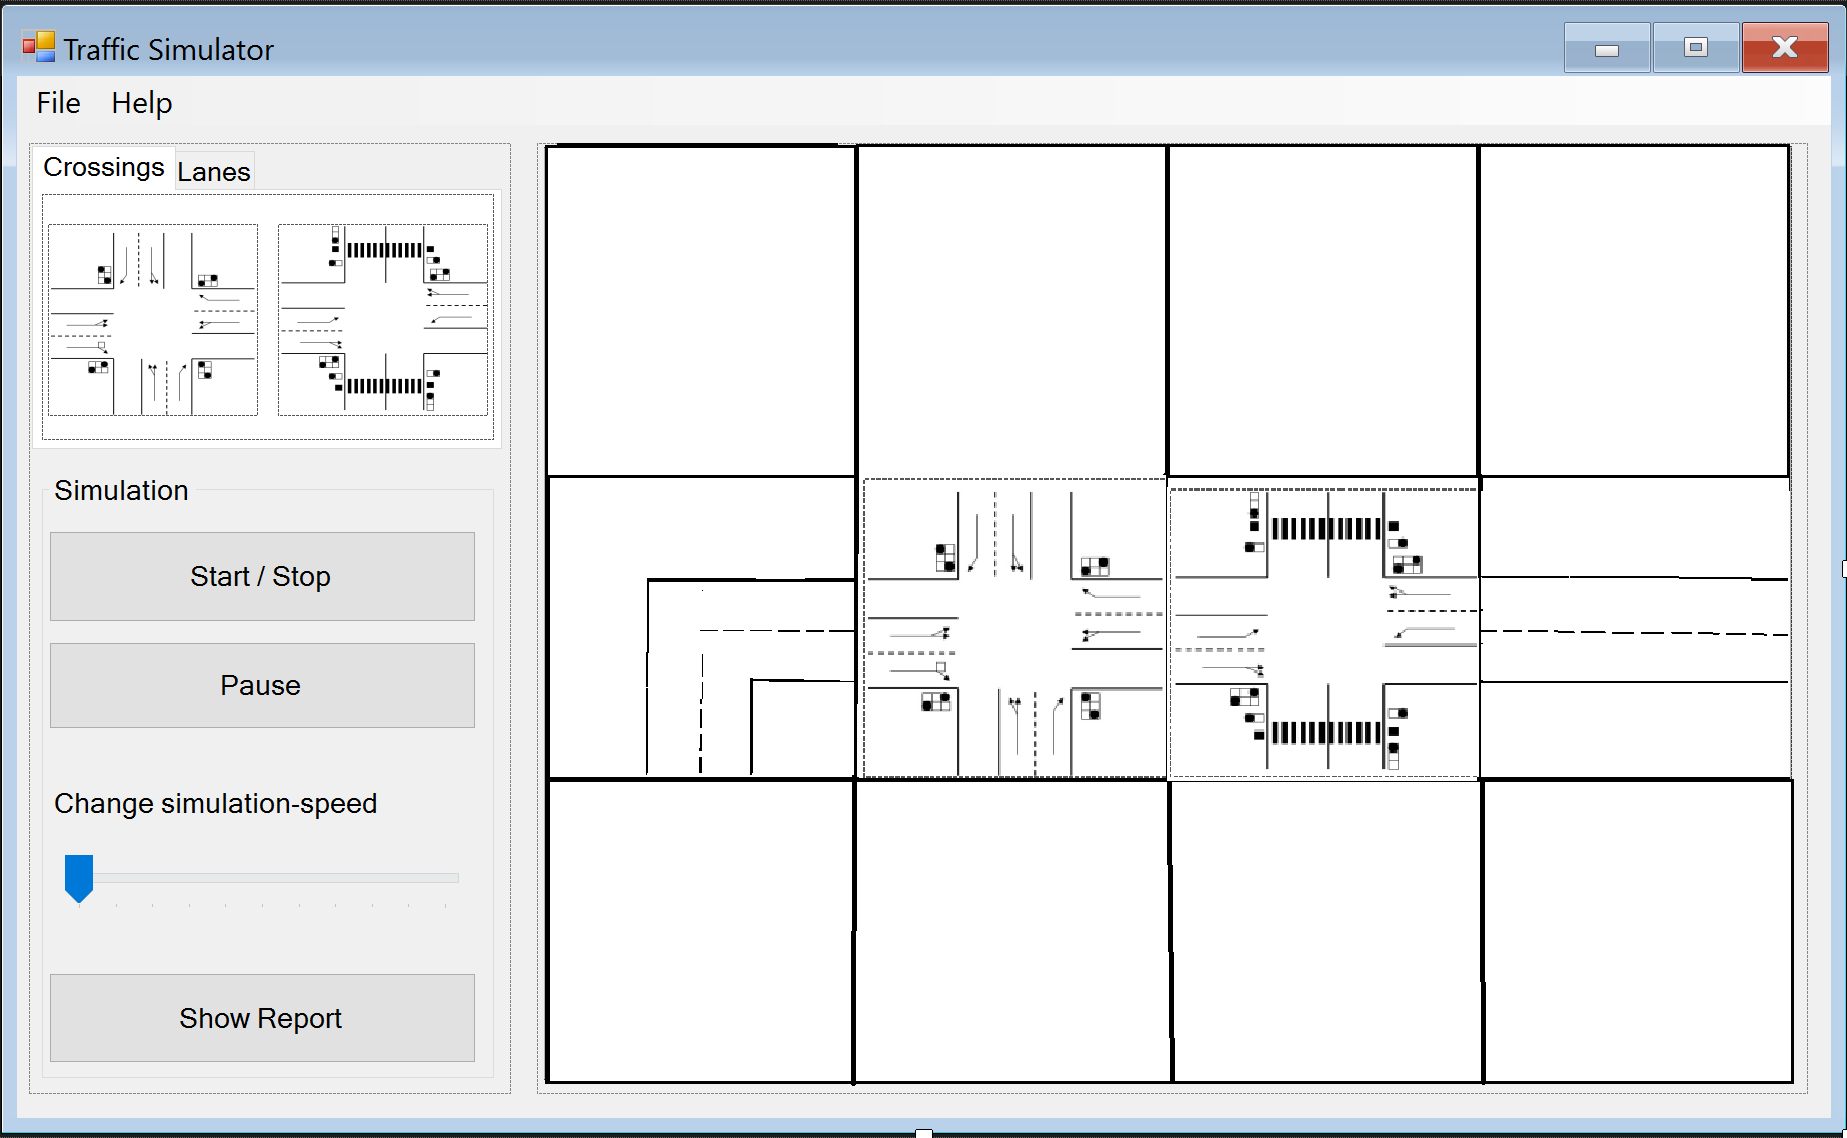
\includegraphics[width=0.8\textwidth]{figures/MainForm}
\end{figure}
\begin{figure}[!ht]
	\caption{Mockup of the Configuration window}
	\label{fig:Configurationwindow}
	\centering
	\includegraphics[width=0.8\textwidth]{figures/configurationForm}
\end{figure}
\begin{tabularx}{\textwidth}{|p{0.5cm}p{2cm}X|}\hline
	Rxx & Code & Specification \\\hline
	R01 & MWS-010 & When the application just started it will create a new grid 4x3\\\hline
	R01 & MWS-020 & The main window has a menubar.\\\hline
	R01 & MWS-020A & The menu bar has the following structure:
	\begin{itemize}[noitemsep,nolistsep]
		\item File
		\begin{itemize}
			\item New
			\item Open
			\item Save
			\item Save As
		\end{itemize}
		\item Help
	\end{itemize}\\\hline
	R01 & MWS-020B & A new simulation can be started by pressing on new, a window will prompt for the width and height for the size of the grid.\\\hline
	R01 & MWS-020C & The manual can be opened by pressing on Help.\\\hline
	R01 & MWS-030 & The window has a sidebar on the left.\\\hline
	R01 & MWS-032 & The sidebar contains all the components described in section \ref*{sec:components}.\\\hline
	R01 & MWS-032A & The component can be added to the grid by dragging it to the desired location.\\\hline
	R01 & MWS-034 & The sidebar contains a button which allows the simulation to start/stop.\\\hline
	R01 & MWS-035 & The sidebar contains a button which allows the simulation to pause.\\\hline
	R01 & MWS-036 & The simulation-speed can be changed by adjusting the slider.\\\hline
	R02 & MWS-038 & In simulation the button "Show report" will generate a report.\\\hline
	R01 & MWS-038A & The report is shown in a new window and contains the current traffic situation including cars and pedestrians.\\\hline
	R01 & MWS-038B & In the report the traffic jams are highlighted.\\\hline
	R01 & MWS-038C & The report can be saved as an image file.\\\hline
\end{tabularx}

To change the amount of time each traffic light is green press right-click on the crossroad and click in the context-menu on "Traffic-light configuration". A new window will pop up which allows to set the time for each group of lanes.

\begin{tabularx}{\textwidth}{|p{0.5cm}p{2cm}X|}\hline
	Rxx & Code & Specification \\\hline
	R01 & MWS-100 & All open incoming lanes have a textbox to specify the amount of traffic coming in.\\\hline
	R01 & MWS-110 & When pressing right-click on any component placed on the grid a context-menu appears which allows to rotate or delete the component.\\\hline
	R01 & MWS-120 & When pressing right-click on a crossroad it gives an option "Traffic-light configuration"\\\hline
	R01 & MWS-120A & A new window will pop-up with a list of all the lane groups.\\\hline
	R01 & MWS-120B & The user can select a lane group and change the amount of time the traffic-light is green.\\\hline
\end{tabularx}

\newpage
\subsection{Components}
\label{sec:components}
\subsubsection{Crossroad}
\begin{figure}
	\centering
	\begin{subfigure}{.5\textwidth}
		\centering
		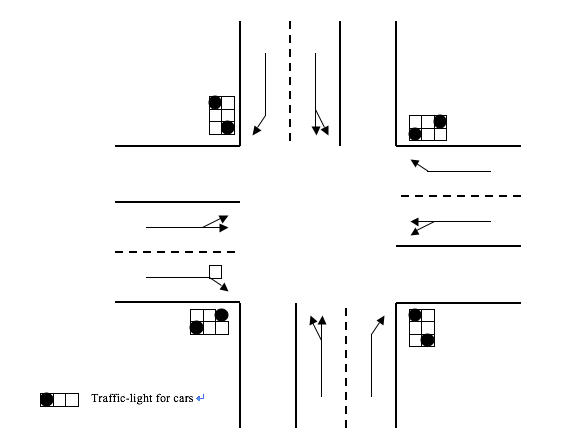
\includegraphics[width=\linewidth]{figures/crosswaya.png}
		\caption{Crossroad without pedestrians.}
		\label{fig:crossa}
	\end{subfigure}%
	\begin{subfigure}{.5\textwidth}
		\centering
		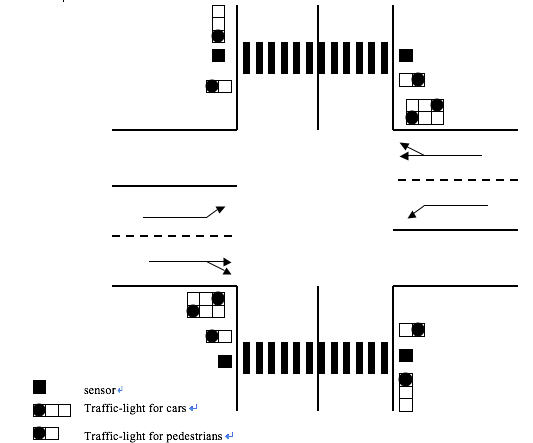
\includegraphics[width=\linewidth]{figures/crosswayb.png}
		\caption{Crossroad with pedestrians.}
		\label{fig:crossb}
	\end{subfigure}
	\caption{Crossways}
	\label{fig:cross}
\end{figure}

\begin{tabularx}{\textwidth}{|p{0.5cm}p{2cm}X|}\hline
	Rxx & Code & Specification \\\hline
	R01 & CWC-010 & All cossways are connected to 4 roads\\\hline
	R01 & CWC-020 & There are 2 different types of crossroads see figure \ref{fig:cross}.\\\hline
	R01 & CWC-020 & Type A crossroad is without pedestrian lane.\\\hline
	R01 & CWC-020A & From each side the crossroad A has 2 incoming lanes and 1 outgoing lane.\\\hline
	R01 & CWC-025 & Type B crossroad is with an pedestrian lane.\\\hline
	R01 & CWC-025A & Type B has from 2 opposite sides a crossroad for pedestrians, which only has 1 incoming lane.\\\hline
	R01 & CWC-030 & Traffic light for cars have the colors red, orange and geen.\\\hline
	R01 & CWC-035 & Traffic light for pedestrians have the colors red and green.\\\hline
	R01 & CWC-040 & Traffic light for cars only turn orange after green.\\\hline
	R01 & CWC-040A & Amount of time for the orange light is fixed, and is set to 2 seconds in normal simulation time.\\\hline
	R01 & CWC-045 & Traffic light for green are set to default for 4 seconds.\\\hline
	R01 & CWC-045A & The amount of time each light group of an crossroad can be changed.\\\hline
	R01 & CWC-050 & The order of the light groups are fixed.\\\hline
	R01 & CWC-050A & When there are no cars or pedestrians on the sensors for the according lightgroup it will be skipped in the simulation.\\\hline
	R01 & CWC-060 & Unconnected incoming lanes have a textbox which allows to change the number of cars comming in when the simulation is running.\\\hline
\end{tabularx}

\newpage
\subsubsection{Road}
\begin{figure}
	\centering
	\begin{subfigure}{.5\textwidth}
		\centering
		\includegraphics{figures/laneaa.png}
		\caption{Straight road.}
		\label{fig:strr}
	\end{subfigure}%
	\begin{subfigure}{.5\textwidth}
		\centering
		\includegraphics{figures/lanebb.png}
		\caption{Curved road.}
		\label{fig:curvedr}
	\end{subfigure}
	\caption{Crossways}
	\label{fig:road}
\end{figure}

\begin{tabularx}{\textwidth}{|p{0.5cm}p{2cm}X|}\hline
	Rxx & Code & Specification \\\hline
	R01 & RCP-010 & There are two types of roads, a straight road and a curved road.\\\hline
	R01 & RCP-020 & All roads have 2 lanes, in both directions.\\\hline
	R01 & RCP-030 & Unconnected incoming lanes have a textbox which allows to change the number of cars comming in when the simulation is running.\\\hline
	R01 & RCP-030A & Just like crossroad see CWC-060.\\\hline
\end{tabularx}

\subsubsection{Car}
\begin{tabularx}{\textwidth}{|p{0.5cm}p{2cm}X|}\hline
	Rxx & Code & Specification \\\hline
	R01 & CAR-010 & All cars run at the same speed, the speed allows 1 car to pass the green light per second.\\\hline
	R01 & CAR-020 & Cars do not collide.\\\hline
	R01 & CAR-020A & Cars hold distance from each other when driving.\\\hline
	R01 & CAR-030 & No cars go through red light.\\\hline
	R01 & CAR-040 & Cars will not go through orange light, in case the car is in front of the traffic light.\\\hline
	R01 & CAR-050 & Cars will take a random direction on the crossroad.\\\hline
	R02 & CAR-060 & Cars accerlate and break at a realistic speed.\\\hline
\end{tabularx}

\subsubsection{Pedestrian}
\begin{tabularx}{\textwidth}{|p{0.5cm}p{2cm}X|}\hline
	Rxx & Code & Specification \\\hline
	R01 & PED-010 & Pedestrians have 50\% change on being at the crosswalk.\\\hline
	R01 & PED-020 & Nothing can be configured of the pedestrians.\\\hline
\end{tabularx}

\newpage
\subsection{Traffic light groups}
\begin{figure}
	\centering
	\begin{subfigure}{.5\textwidth}
		\centering
		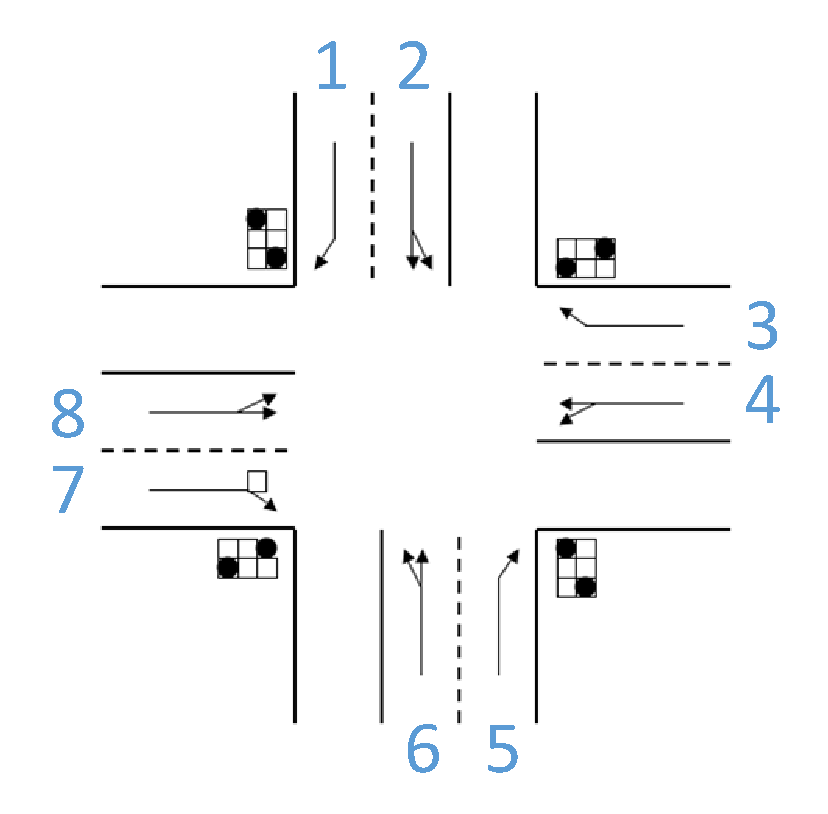
\includegraphics[width=0.8\textwidth]{figures/CrossroadAL.pdf}
		\caption{Crossroad A incoming lane numbers.}
		\label{fig:cral}
	\end{subfigure}%
	\begin{subfigure}{.5\textwidth}
		\centering
		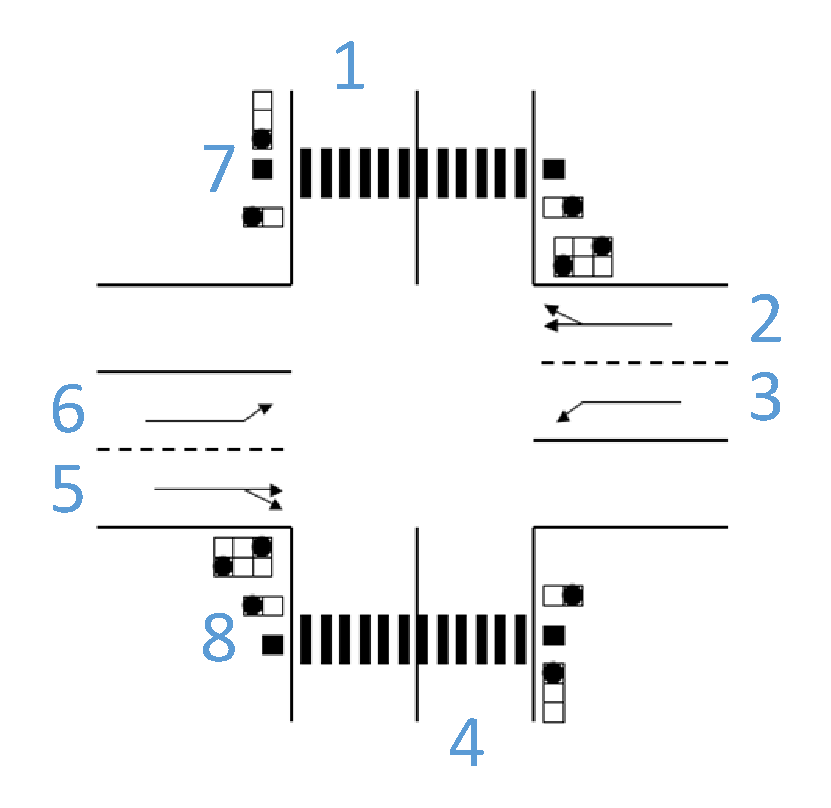
\includegraphics[width=0.8\textwidth]{figures/CrossroadBL.pdf}
		\caption{Crossroad B incoming lane numbers.}
		\label{fig:crbl}
	\end{subfigure}
	\caption{Crossways}
	\label{fig:tlg}
\end{figure}

The group of lanes which have green light at the same moment are defined in this section. The traffic lights follow the order as defined in this document, Traffic lights will skip a light group if no cars are present on the group of lanes.

\subsubsection{Crossroad A}
\begin{tabularx}{\textwidth}{|p{0.6cm}p{4cm}X|p{0.6cm}p{4cm}X|}\hline
	ID & Image & Lanes & ID & Image & Lanes \\\hline
	A1 &  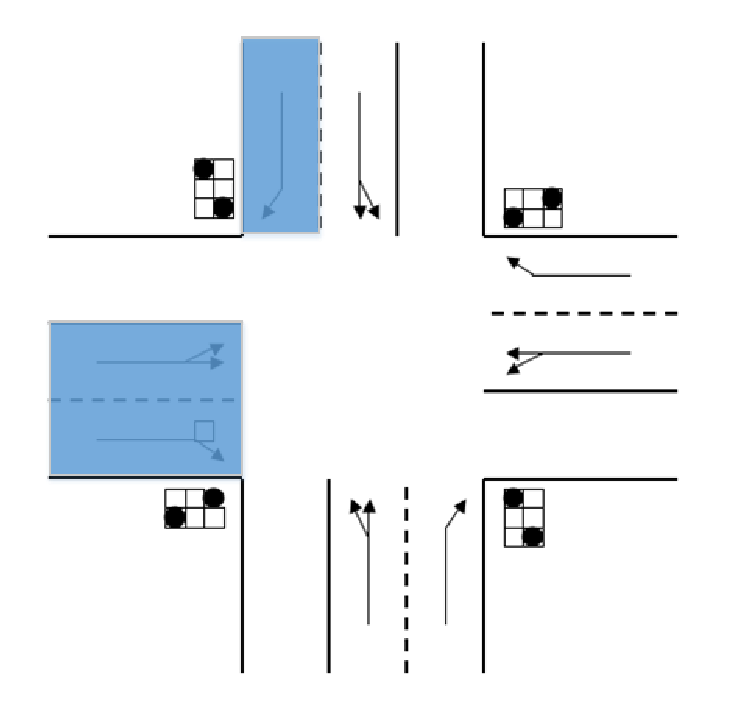
\includegraphics[width=4cm]{figures/CrossroadA1.pdf} & 1, 7, 8 &
	A2 &  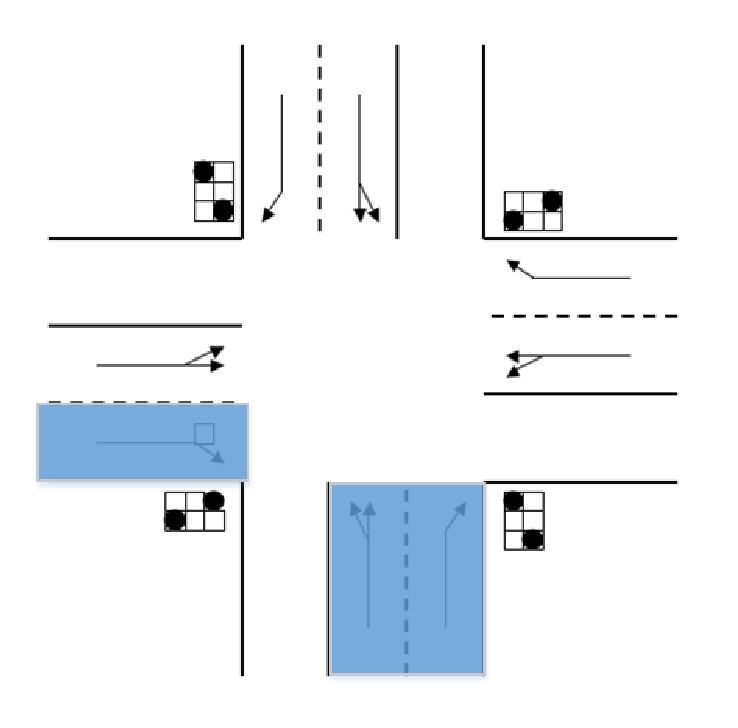
\includegraphics[width=4cm]{figures/CrossroadA2.pdf} & 5, 6, 7 \\\hline
	A3 &  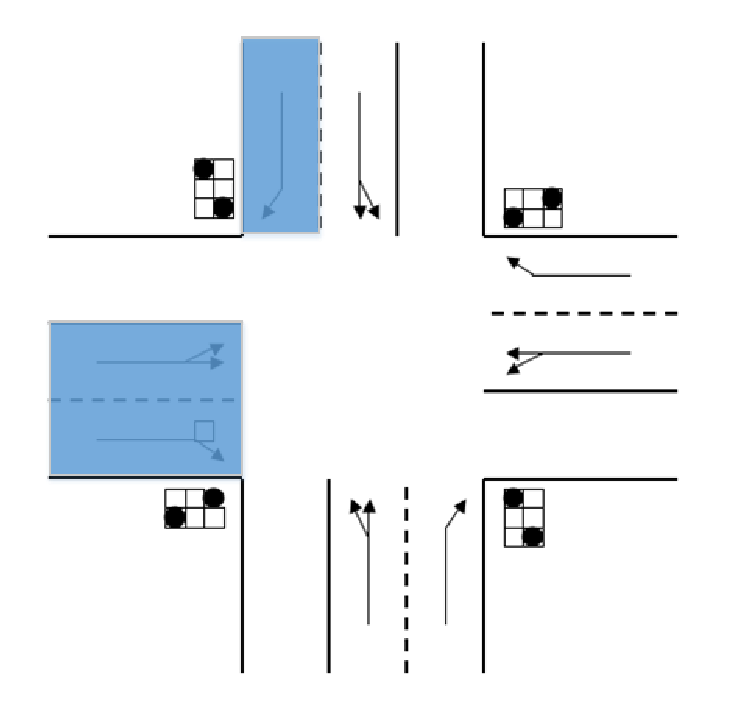
\includegraphics[width=4cm]{figures/CrossroadA3.pdf} & 3, 4, 5 &
	A4 &  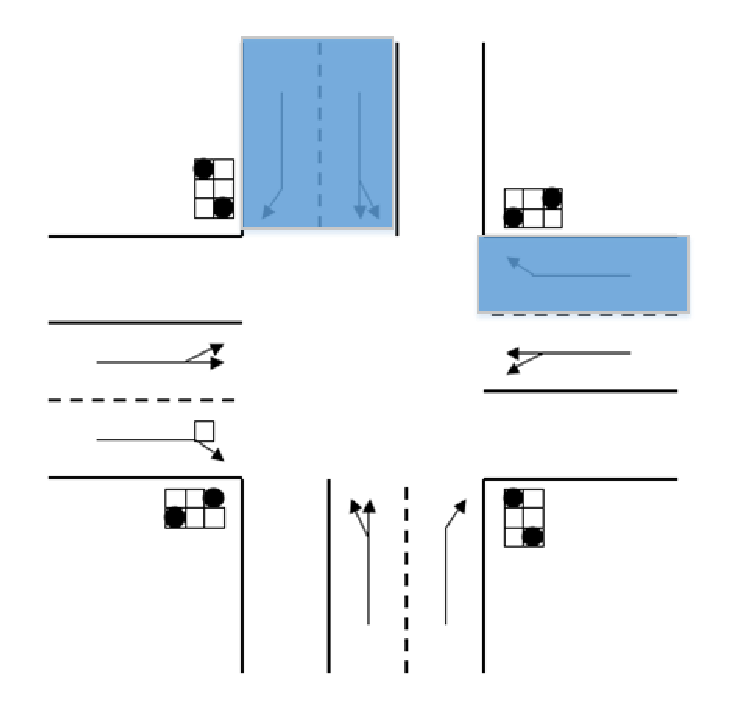
\includegraphics[width=4cm]{figures/CrossroadA4.pdf} & 1, 2, 3 \\\hline
\end{tabularx}

\subsubsection{Crossroad B}
\begin{tabularx}{\textwidth}{|p{0.6cm}p{4cm}X|p{0.6cm}p{4cm}X|}\hline
	ID & Image & Lanes & ID & Image & Lanes \\\hline
	B1 &  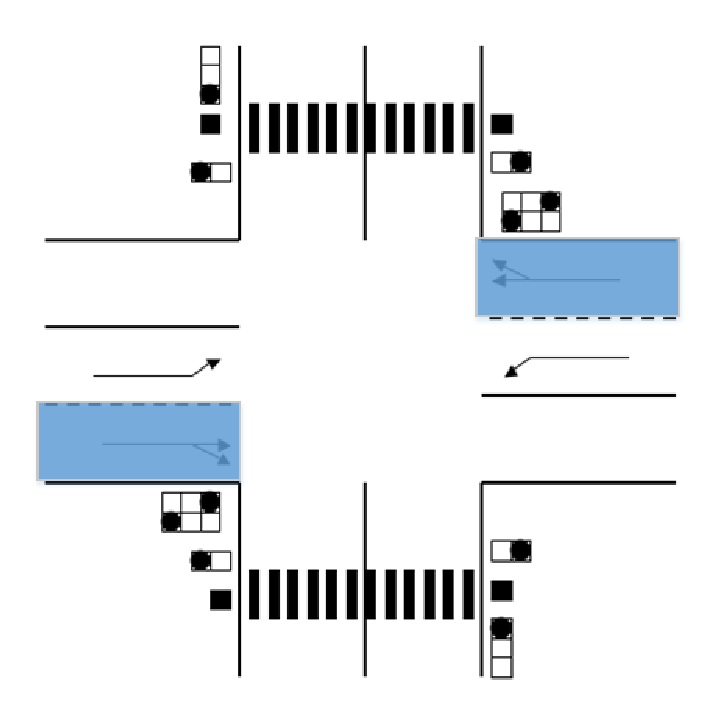
\includegraphics[width=4cm]{figures/CrossroadB1.pdf} & 2, 5 &
	B2 &  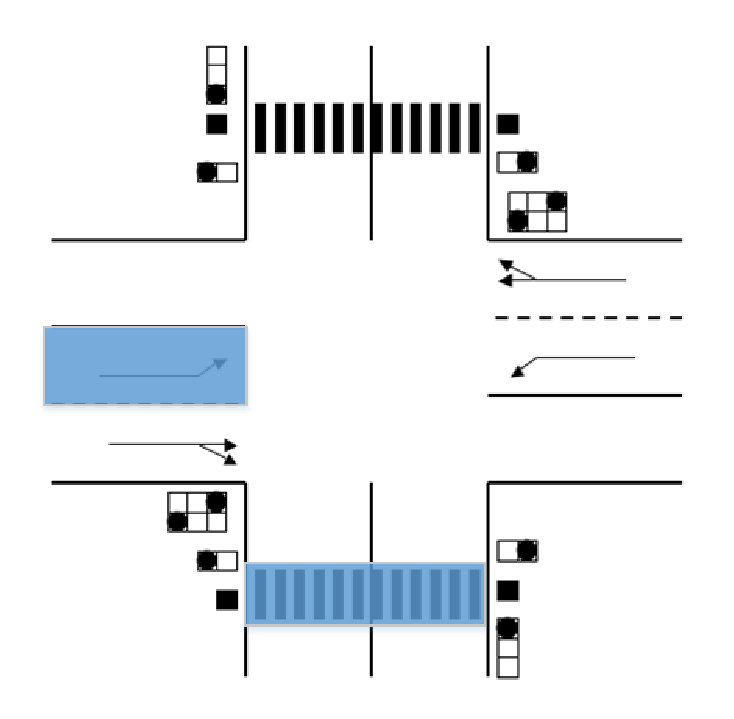
\includegraphics[width=4cm]{figures/CrossroadB2.pdf} & 6, 8 \\\hline
	B3 &  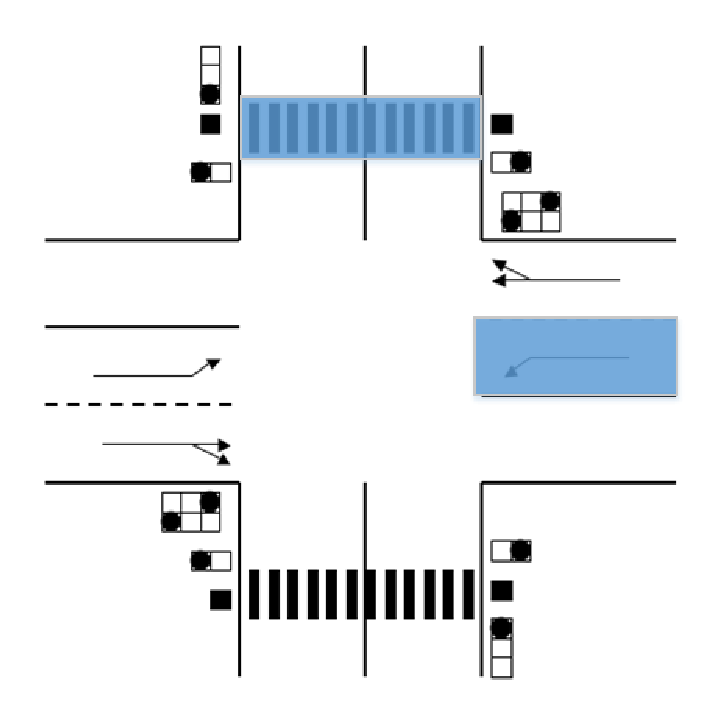
\includegraphics[width=4cm]{figures/CrossroadB3.pdf} & 3, 7 &
	B4 &  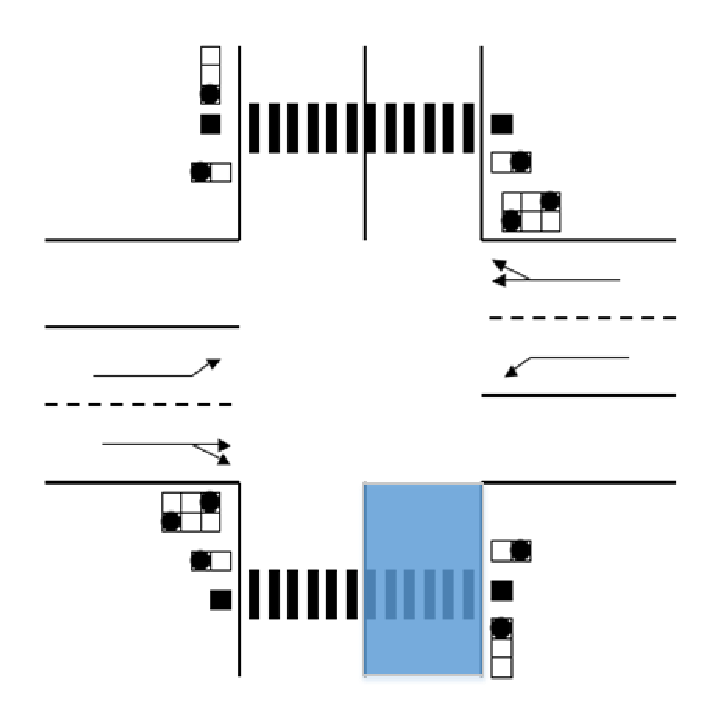
\includegraphics[width=4cm]{figures/CrossroadB4.pdf} & 4 \\\hline
	B5 &  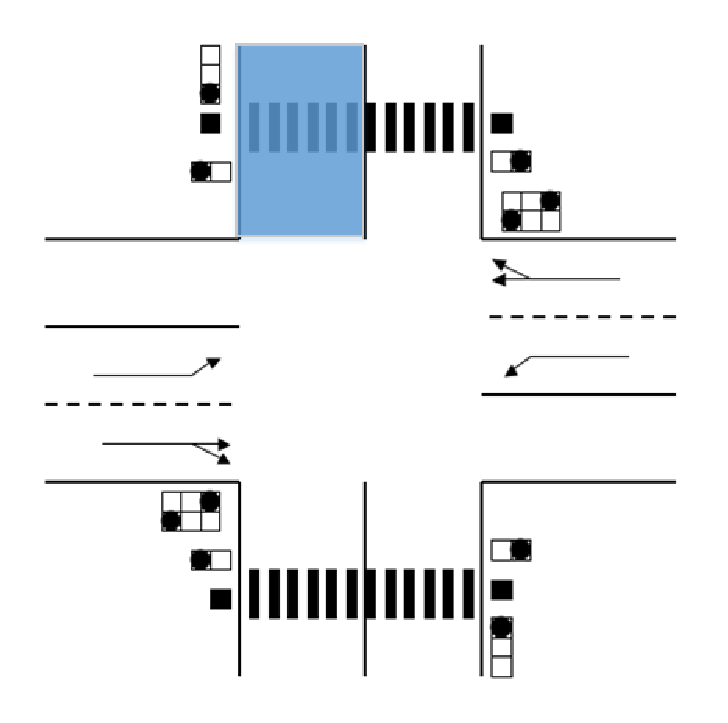
\includegraphics[width=4cm]{figures/CrossroadB5.pdf} & 1 & & & \\\hline
\end{tabularx}
